\documentclass[conference]{IEEEtran}
\IEEEoverridecommandlockouts
% The preceding line is only needed to identify funding in the first footnote. If that is unneeded, please comment it out.
\usepackage{cite}
\usepackage{amsmath,amssymb,amsfonts}
\usepackage{algorithmic}
\usepackage{graphicx}
\usepackage{textcomp}
\usepackage[pdftex,dvipsnames]{xcolor}
\setlength {\marginparwidth }{2cm}
\usepackage[colorinlistoftodos,prependcaption,textsize=tiny]{todonotes}
\def\BibTeX{{\rm B\kern-.05em{\sc i\kern-.025em b}\kern-.08em
    T\kern-.1667em\lower.7ex\hbox{E}\kern-.125emX}}

\begin{document}
\documentclass[main.tex]{subfiles}

\begin{document}


\begin{abstract}
Se ecualizó una señal en un enlace digital basándose en el 
esquema de filtrado de inversión de sistemas. Se implementó
NLMS, justificando la elección de los parámetros, consiguiendo
minimizar el bit error rate, la tasa de errores. Luego se buscó de manera exitosa 
implementar RLS, consiguiendo aún mejores resultados para el problema.
\end{abstract}


\section{Introducción}
Se buscó ecualizar una señal en un enlace digital de comunicaciones. 
Los datos consistían en una secuencia de datos pseudoaleatoria 
codificada por Manchester, muestreada a una frecuencia de sampleo
 de 4 kHz a razón de 250 bps. Ante estas características, cada bit consiste de 
 16 muestras según la codificación mencionada. El canal, en este caso, conocido, 
 modificaba la señal dependiendo del posicionamiento
 aleatorio de dos pares de polos conjugados. En lo que respecta a estacionaridad, 
 el canal carece de la misma debido a sus características cambiantes en el tiempo.
La principal dificultad consistía entonces en la variabilidad del canal. En las 
siguientes figuras se puede notar el efecto de lo mencionado, siendo la 
señal en azul los bits enviados y en naranja lo recibido. \newline

\begin{figure}[H]
    \centering
    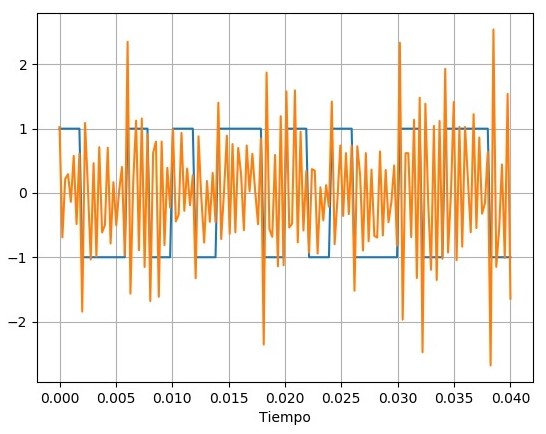
\includegraphics[scale=0.5]{imagenes/1.jpeg}
\end{figure}
\begin{figure}[H]
    \centering
    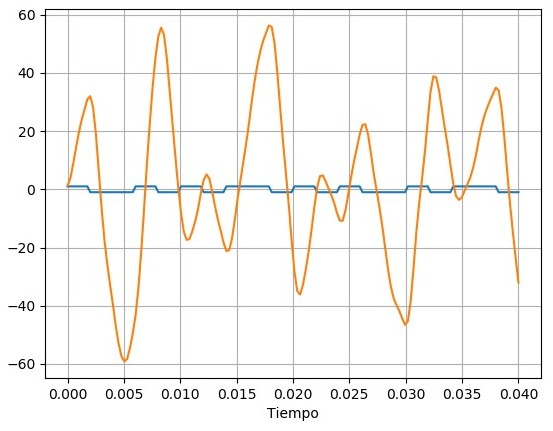
\includegraphics[scale=0.5]{imagenes/2.jpeg}
\end{figure}
\begin{figure}[H]
    \centering
    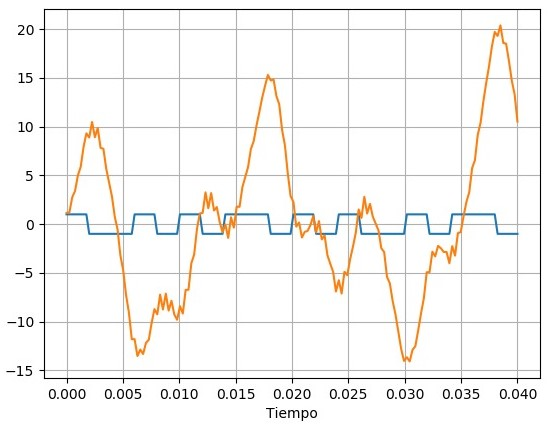
\includegraphics[scale=0.5]{imagenes/3.jpeg}\\
    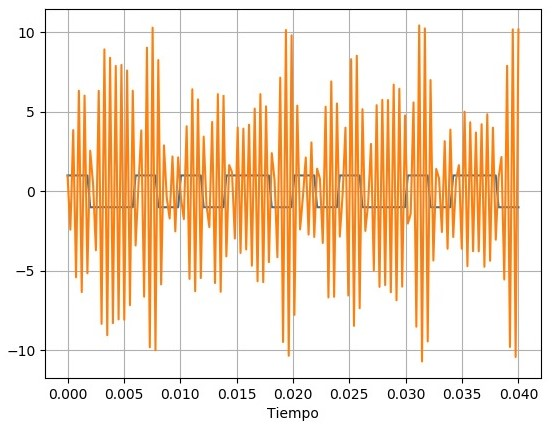
\includegraphics[scale=0.5]{imagenes/4.jpeg}
    \caption{Señales obtenidas en el receptor, al pasar por el canal.}
\end{figure}

El proyecto consiste en aplicar un algoritmo de filtrado adaptativo
 para recuperar la señal transmitida asumiendo que no se conoce la entrada, 
 lo que simularía un enlace digital de comunicaciones.
 Un esquema de lo mencionado
se puede ver en la siguiente figura.

\begin{figure}[H]
    \centering
    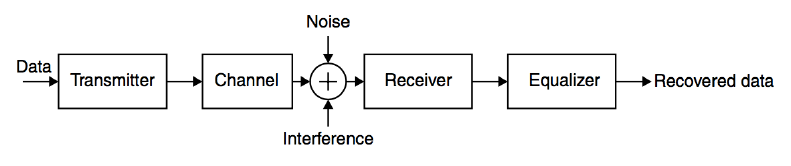
\includegraphics[scale=0.5]{imagenes/preblock.png}
    \caption{Esquema del enlace digital.}
\end{figure}

Como criterio de validación del algoritmo como así de sus parámetros, se calculó el bit error rate (BER), la
cantidad de bits errados por unidad de tiempo.



\end{document}
\section{Ecualización Adaptativa por Inversión de Sistemas}
\todo{que onda el nombre de esta seccion xxdxdx}

El objetivo del proyecto es invertir los efectos del canal 
-el sistema desconocido- mediante el esquema de filtrado
adaptativo conocido como inversión de sistemas. El diagrama se muestra 
a continuación:

\begin{figure}[h]
    \centering
    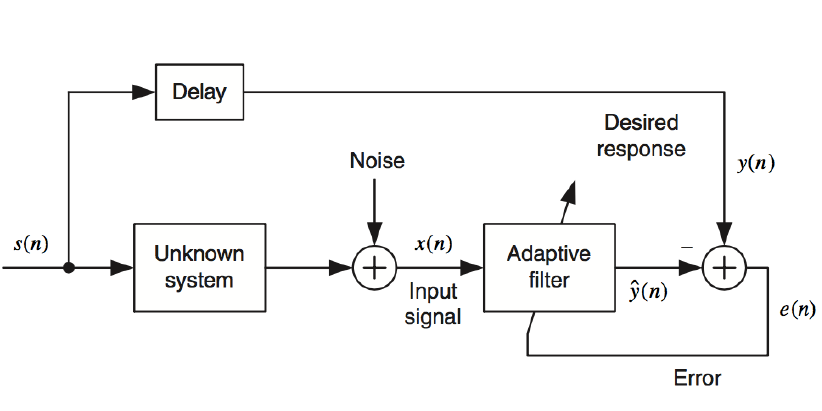
\includegraphics[scale=0.5]{imagenes/block.PNG}
    \caption{Inversión de sistemas.}
\end{figure}

En principio se asume que el ruido del canal 
es incorrelacionado con $s(n)$.
El filtrado funciona de la siguiente manera, se tiene 
la señal de entrada $s(n)$, que se transmite por el sistema
desconocido -el canal ya mencionado-, cuya salida es la señal 
$x(n)=u(n)$, que es la entrada al filtro adaptativo, de donde se obtiene
$\hat{y}(n)$. Realimentando la señal de error $e(n)$
al filtro adaptativo se maximiza la correlación entre la salida del 
filtro y la señal deseada $y(n)=d(n)$.
Opcionalmente, a su vez, se puede colocar un delay, retrasando la señal al obtener 
$d(n)$ para compensar el delay propio del sistema.\newline
Con ésto se consigue una salida con una respuesta en frecuencia inversa
al sistema desconocido, lo que anula su efecto.\newline
Sin embargo, en un enlace digital el receptor no conoce la respuesta deseada, por lo que
este esquema no es de utilidad. La solución consiste en utilizar 
una secuencia de entrenamiento, una respuesta deseada $d(n)$ preacordada entre 
emisor y receptor.
El diagrama de bloques completo se observa en la figura siguiente:
\begin{figure}[h]
    \centering
    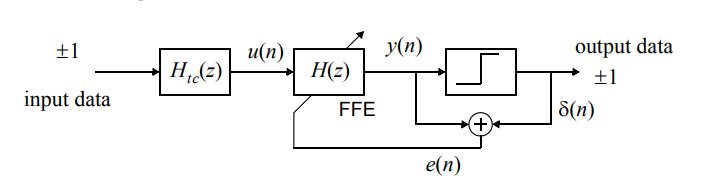
\includegraphics[scale=0.4]{imagenes/esquema.PNG}
    \caption{Diagrama de bloques con decision-directed feedback.}
\end{figure}
Luego del período de entrenamiento inicial los coeficientes del ecualizador pueden ser
 continuamente ajustados con un decision-directed feedback. De esta manera, 
 la señal de error $e(n)=d(n)-y(n)$ se deriva del último (no necesariamente correcto) 
 bit estimado de la secuencia transmitida $u(n)$. Cabe aclarar que 
 la estimación depende de las 16 muestras que componen cada bit, y se implementó la óptima.


\todo[]{Análisis del Canal}

\documentclass[main.tex]{subfiles}

\begin{document}

\section{Filtro Adaptativo}
Al momento de elegir el algoritmo que se implementó para el filtro, 
se analizaron varias alternativas, entre ellas LMS, NLMS, VS-LMS y Sign LMS.
En primer lugar, los algoritmos Sign LMS, entre ellos, sign-error, sign-data
y sign-sign fueron descartados ya que el baud rate de la señal era de 250bps,
cabe recordar que esta variante de LMS es de utilidad para ecualizar canales de
comunicación digital de alta velocidad. En segundo lugar y  luego de analizar 
los resultados obtenidos y las conclusiones propuestas por Bismor \cite{bismor},
se decidió no implementar VS-LMS. En las palabras de los autores: 
"no hay algoritmo VS-LMS que sea tan versátil, fácil de implementar y adecuado 
para aplicaciones en tiempo real como el NLMS".\newline
Esta observación, si bien descarta la implementación de VS-LMS, 
plantea un último debate respecto a si corresponde utilizar LMS o NLMS. 
Se consideró entonces, analizar el parámetro de paso que se utilizaría para LMS. 
Se recuerda que el paso para que converja LMS está dado por
\begin{equation}
    0<\mu<\frac{2}{\lambda_\text{máx}}
\end{equation}
en donde $\lambda_\text{máx}$ es el autovalor más grande de $R$, la matriz de 
autocorrelación de $u(n)$. En la medida en que el  $\mu$ elegido se acerque 
al valor máximo, la velocidad de convergencia aumenta, pero así también el desajuste $\mathscr{M}$.
Por el contrario, al disminuir el paso, la convergencia se ralentiza, y disminuye $\mathscr{M}$. 
Se trata de una relación de compromiso entre la velocidad de convergencia y el desajuste.
Se realizaron 5000 simulaciones y se calculó el $\mu_\text{máx}$ para cada una de ellas.
Se muestra a continuación un histograma con la frecuencia de aparición del paso máximo, 
en función de este y los $\mu_\text{máx}$ en función del número de simulación.
\begin{figure}[H]
    \centering
    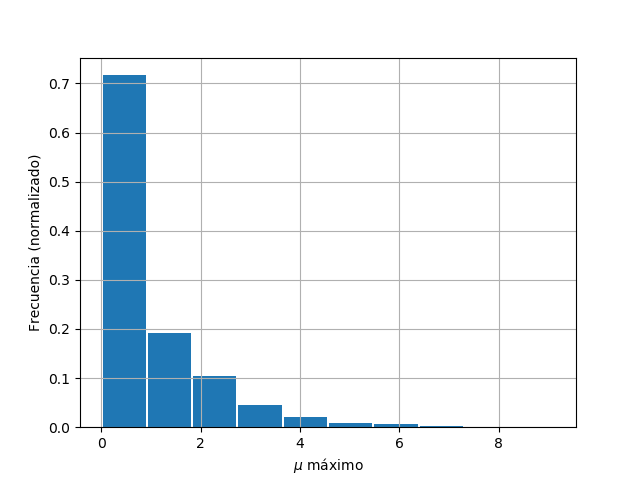
\includegraphics[scale=0.5]{imagenes/lms_mus_hist.png}
    \caption{Frecuencias de $\mu_\text{máx}$ en función del mismo.}
\end{figure}
\begin{figure}[H]
    \centering
    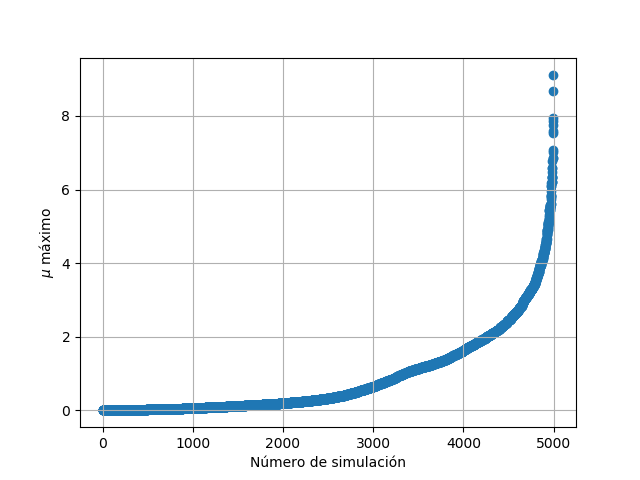
\includegraphics[scale=0.5]{imagenes/lms_mus_scatter.png}
    \caption{$\mu_\text{máx}$ en función del número de simulación.}
\end{figure}

El valor del parámetro de paso varía entre valores cercanos a 0 y mayores a 8, 
ya que las energías de la señal de entrada no están acotadas debido a las características 
del canal. Lo último presenta un problema al elegir el $\mu$ conveniente para la situación real,
puesto que si se elige un paso pequeño, tardará de manera considerable cuando el $\mu_\text{máx}$ sea alto;
y si se decide por un $\mu$ mayor, divergirá en los otros casos. \newline
Debido a lo expuesto anteriormente, se decidió no utilizar LMS, en pos de que no diverja el algoritmo. 
Esto se logró utilizando NLMS, pues lo que se introduce es un parámetro de paso variable, que depende
de la energía de la señal de entrada, por lo que la misma ya no es un problema.

\subsection*{NLMS}
\subsection*{Implementación}
\subsubsection*{Orden del filtro}
Como se mencionó en secciones anteriores, el canal es, si bien aleatorio, conocido, por 
lo que se pudo observar analizándolo que contaba con dos pares de polos conjugados, 4 polos.
Resulta entonces trivial la observación que con un filtro FIR de orden 4, los efectos 
de las singularidades se verían neutralizados. Se implementó entonces NLMS, y se realizó
una simulación de Montecarlo del bit error rate (BER) para órdenes de filtro entre 4, 5 y 6, en función del parámetro 
$\mu$.

\begin{figure}[H]
    \centering
    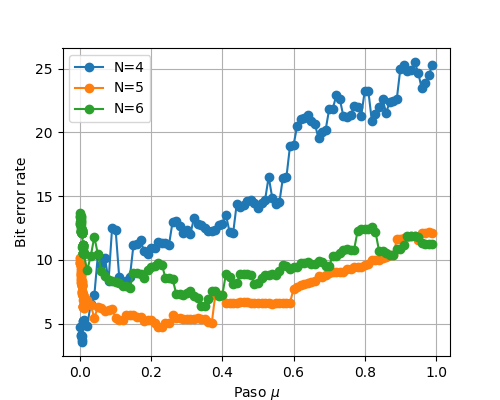
\includegraphics[scale=0.6]{imagenes/N_filter.png}
    \caption{Bit error rate en función de $\mu$ para orden 4, 5 y 6 del filtro.}
\end{figure}

Se observa que para valores de $\mu$ pequeños, el algoritmo mantiene un BER bajo 
para orden 4, desestabilizándose para pasos más grandes; no así ocurre con orden 5, 
que si bien tiene un mayor BER para valores bajos, tiene resultados más consistentes
para valores mayores de $\mu$. A su vez, este orden obtiene mejores resultados que un 
filtro de sexto orden. Con todo, el orden del filtro elegido fue 5.

\subsubsection*{Delay}
En lo que respecta al delay, bloque del esquema de inversión de sistemas, 
figura \ref{inversion-de-sistemas}, el retardo funciona como una compensación del delay real
del filtro y del canal. Además, es sólo utilizado para la secuencia de entrenamiento, para obtener la señal deseada.
En primer lugar se acotó el valor del delay entre 0-4 por el orden ideal del filtro, 
luego realizó un Montecarlo para estos valores de delay, donde nuevamente se
graficó el BER en función del parámetro de paso. Obteniendo una mejor tasa de error 
para el caso de delay unitario por lo que fue elegido.
\begin{figure}[H]
    \centering
    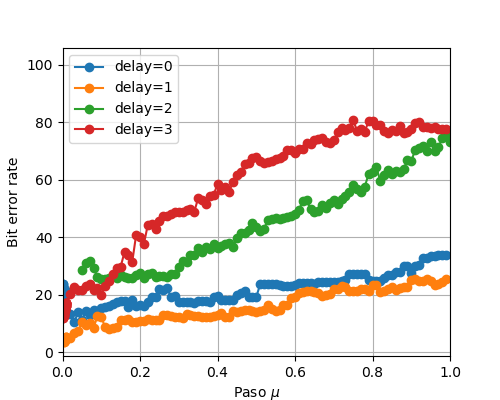
\includegraphics[scale=0.6]{imagenes/delay.png}
    \caption{Bit error rate en función de $\mu$ para delays entre 0-4.}
\end{figure}

\subsubsection*{Paso $\mu$}
De manera análoga, con base en ambos gráficos, se eligió un paso $\mu=0.005$; el valor
para el cual tanto para un  delay unitario, como para un filtro de quinto orden
el BER obtenido era menor al $5\%$.


\end{document}

\section*{Acknowledgment}

The preferred spelling of the word ``acknowledgment'' in America is without 
an ``e'' after the ``g''. Avoid the stilted expression ``one of us (R. B. 
G.) thanks $\ldots$''. Instead, try ``R. B. G. thanks$\ldots$''. Put sponsor 
acknowledgments in the unnumbered footnote on the first page.

\section*{References}

Number footnotes separately in superscripts. Place the actual footnote at 
the bottom of the column in which it was cited. Do not put footnotes in the 
abstract or reference list. Use letters for table footnotes.

\todo{shanmugan;los dos papers}
\begin{thebibliography}{00}
    % \ref{b1}
\bibitem{b1} G. Eason, B. Noble, and I. N. Sneddon, ``On certain integrals of Lipschitz-Hankel type involving products of Bessel functions,'' Phil. Trans. Roy. Soc. London, vol. A247, pp. 529--551, April 1955.
\bibitem{b2} J. Clerk Maxwell, A Treatise on Electricity and Magnetism, 3rd ed., vol. 2. Oxford: Clarendon, 1892, pp.68--73.
\bibitem{b3} I. S. Jacobs and C. P. Bean, ``Fine particles, thin films and exchange anisotropy,'' in Magnetism, vol. III, G. T. Rado and H. Suhl, Eds. New York: Academic, 1963, pp. 271--350.
\bibitem{b4} K. Elissa, ``Title of paper if known,'' unpublished.
\bibitem{b5} R. Nicole, ``Title of paper with only first word capitalized,'' J. Name Stand. Abbrev., in press.
\bibitem{b6} Y. Yorozu, M. Hirano, K. Oka, and Y. Tagawa, ``Electron spectroscopy studies on magneto-optical media and plastic substrate interface,'' IEEE Transl. J. Magn. Japan, vol. 2, pp. 740--741, August 1987 [Digests 9th Annual Conf. Magnetics Japan, p. 301, 1982].
\bibitem{b7} M. Young, The Technical Writer's Handbook. Mill Valley, CA: University Science, 1989.
\end{thebibliography}
\vspace{12pt}
\color{red}
IEEE conference templates contain guidance text for composing and formatting conference papers. Please ensure that all template text is removed from your conference paper prior to submission to the conference. Failure to remove the template text from your paper may result in your paper not being published.

\end{document}
